\documentclass[../main.tex]{subfiles}

\begin{document}

\section{Results}
\justify

This section presents the experimental results from both the simulation evaluation and the real-world flight trials. Results are reported at two levels: episode-level success rate (the drone completes the full 15\,m corridor without any collision) and per-obstacle avoidance probability. All conditions were evaluated over 50 episodes per density configuration. The full episode-by-episode datasets for both simulation and real-world trials are available in Appendix A.

The per-obstacle avoidance probability is estimated as the maximum likelihood estimator (MLE) of the truncated geometric distribution: $\hat{p} = N_{\text{avoided}} / (N_{\text{avoided}} + N_{\text{fail}})$, where $N_{\text{avoided}}$ is the total number of trees successfully avoided across all episodes and $N_{\text{fail}}$ is the total number of failed episodes. This treats each tree encounter as an independent Bernoulli trial with success probability $p$, with each episode stopping at the first collision. The 95\,\% confidence intervals are computed as $\hat{p} \pm 1.96\,\mathrm{SE}$, where $\mathrm{SE} = \sqrt{\hat{p}(1-\hat{p})/N}$ and $N = N_{\text{avoided}} + N_{\text{fail}}$. Episode-level success rates are treated as binomial proportions and use the same normal-approximation formula with $N$ equal to the number of episodes.

\subsection{Training Stability}

Figure \ref{fig:tensorboard_training} shows the PPO training curves recorded in TensorBoard. In all three subplots the x-axis is training timesteps. Training proceeds in two curriculum stages: a sparse stage (2-tree corridor) followed by a dense stage (3-tree corridor), with the policy checkpoint from the sparse stage used to initialise the dense stage. Subplot (a) shows episode success rate --- the fraction of episodes completed without a collision (y-axis) --- climbing steadily and plateauing, reaching up to 92\,\% during the dense stage. Subplot (b) shows value loss --- the PPO critic's value-prediction error (y-axis) --- falling and stabilising, confirming that the PPO critic's value estimates converge without collapse \cite{Schulman2017}. Subplot (c) shows mean episode length --- the average number of steps before the episode ends (y-axis) --- increasing over the course of training, indicating that the drone survives progressively longer in the corridor as it learns to avoid early collisions.

\begin{figure}[H]
    \centering
    \begin{minipage}[t]{0.45\textwidth}
        \centering
        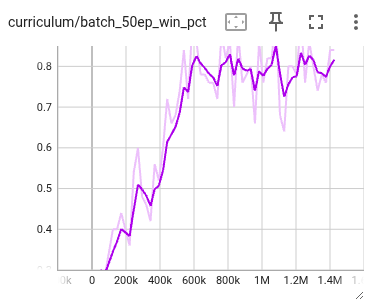
\includegraphics[width=\textwidth]{figures/success-rate.png}
        \small (a) Episode success rate (y-axis) vs.\ training timesteps (x-axis) --- the y-axis is the fraction of episodes completed without a collision; it rises steadily, reaching up to 92\,\% in the dense stage
    \end{minipage}
    \hfill
    \begin{minipage}[t]{0.45\textwidth}
        \centering
        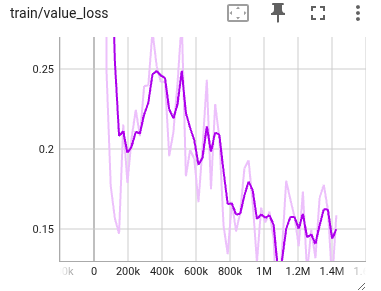
\includegraphics[width=\textwidth]{figures/value-loss.png}
        \small (b) Value loss (y-axis) vs.\ training timesteps (x-axis) --- the y-axis is the PPO critic's value-prediction error; it falls and stabilises, confirming critic convergence
    \end{minipage}
    \vspace{6pt}

    \begin{minipage}[t]{0.45\textwidth}
        \centering
        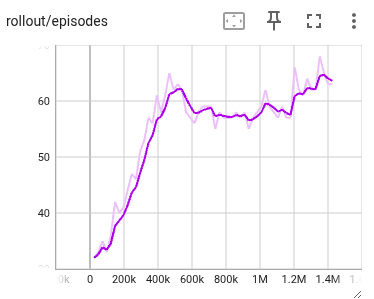
\includegraphics[width=\textwidth]{figures/episode-length.png}
        \small (c) Mean episode length (y-axis) vs.\ training timesteps (x-axis) --- the y-axis is the average number of steps before the episode ends; it grows as the agent survives progressively longer before colliding
    \end{minipage}
    \caption{PPO training curves from TensorBoard (x-axis: training timesteps). Training proceeds in two sequential curriculum stages (sparse then dense); the dense stage is initialised from the sparse-stage checkpoint.}
    \label{fig:tensorboard_training}
\end{figure}

\subsection{Simulation Results}

The trained policy was evaluated over 100 episodes in simulation: 50 sparse (2 trees in corridor) and 50 dense (3 trees in corridor). Table \ref{tab:sim_results} summarises the results. Figure \ref{fig:sim_bar} visualises the episode-level and per-obstacle success rates across both density conditions.

\vspace{6pt}
\begin{table}[H]
\centering
\caption{Simulation evaluation results across density conditions.}
\label{tab:sim_results}
\resizebox{\textwidth}{!}{%
\begin{tabular}{|l|c|c|c|c|c|}
\hline
\textbf{Condition} & \textbf{Episodes} & \textbf{Episode Success Rate} & \textbf{95\% CI} & \textbf{Per-Obs.\ $\hat{p}$} & \textbf{95\% CI} \\
\hline
Sparse (2 trees) & 50 & 94.00\% & {[87.4,\,100]\%} & 97.00\% & {[93.7,\,100]\%} \\
Dense (3 trees) & 50 & 84.00\% & {[73.8,\,94.2]\%} & 94.67\% & {[91.1,\,98.3]\%} \\
\hline
\textbf{Total} & \textbf{100} & \textbf{89.00\%} & \textbf{[82.9,\,95.1]\%} & \textbf{95.60\%} & \textbf{[93.1,\,98.1]\%} \\
\hline
\end{tabular}%
}
\end{table}

\begin{figure}[H]
\centering
\begin{tikzpicture}
\begin{axis}[
    ybar,
    bar width=28pt,
    width=\textwidth,
    height=9cm,
    ylabel={Success Rate (\%)},
    ymin=0, ymax=130,
    ytick={0,20,40,60,80,100},
    xtick=data,
    symbolic x coords={Sparse, Dense, Total},
    legend style={at={(0.98,0.98)}, anchor=north east},
    nodes near coords,
    nodes near coords align={vertical},
    every node near coord/.append style={font=\small, text=black, anchor=north, yshift=-4pt},
    enlarge x limits=0.25,
    grid=major,
    grid style={dashed,gray!40},
]
\addplot+[fill=lightblue, draw=black,
    error bars/.cd, y dir=both, y explicit,
    error bar style={draw=black, line width=0.8pt}] coordinates {
    (Sparse, 94.00) +- (0, 6.58) (Dense, 84.00) +- (0, 10.16) (Total, 89.00) +- (0, 6.13)
};
\addplot+[fill=lavenderpurple, draw=black,
    error bars/.cd, y dir=both, y explicit,
    error bar style={draw=black, line width=0.8pt}] coordinates {
    (Sparse, 97.00) +- (0, 3.34) (Dense, 94.67) +- (0, 3.59) (Total, 95.60) +- (0, 2.54)
};
\legend{Episode Success, Per-Obs.\ $\hat{p}$}
\end{axis}
\end{tikzpicture}
\caption{Simulation episode-level and per-obstacle success rates by tree density. Error bars show 95\,\% confidence intervals.}
\label{fig:sim_bar}
\end{figure}

The agent achieved a 94.00\% episode success rate in sparse conditions and 84.00\% in dense conditions. The per-obstacle success rates were consistently higher than the episode-level rates in both conditions, reflecting that the agent frequently avoided most trees in an episode even when one collision ultimately terminated the run.

\subsection{Real-World Results}

The same policy was deployed without fine-tuning on the physical Holybro S500 V2 platform. A total of 100 real-world flights were conducted: 50 sparse and 50 dense. Table \ref{tab:real_results} summarises the results. Figure \ref{fig:real_bar} shows the success rates by condition.

\vspace{6pt}
\begin{table}[H]
\centering
\caption{Real-world flight results across density conditions.}
\label{tab:real_results}
\resizebox{\textwidth}{!}{%
\begin{tabular}{|l|c|c|c|c|c|}
\hline
\textbf{Condition} & \textbf{Episodes} & \textbf{Episode Success Rate} & \textbf{95\% CI} & \textbf{Per-Obs.\ $\hat{p}$} & \textbf{95\% CI} \\
\hline
Sparse (2 trees) & 50 & 74.00\% & {[61.8,\,86.2]\%} & 86.46\% & {[79.6,\,93.3]\%} \\
Dense (3 trees) & 50 & 70.00\% & {[57.3,\,82.7]\%} & 88.64\% & {[83.2,\,94.1]\%} \\
\hline
\textbf{Total} & \textbf{100} & \textbf{72.00\%} & \textbf{[63.2,\,80.8]\%} & \textbf{87.72\%} & \textbf{[83.5,\,92.0]\%} \\
\hline
\end{tabular}%
}
\end{table}

\begin{figure}[H]
\centering
\begin{tikzpicture}
\begin{axis}[
    ybar,
    bar width=28pt,
    width=\textwidth,
    height=9cm,
    ylabel={Success Rate (\%)},
    ymin=0, ymax=120,
    ytick={0,20,40,60,80,100},
    xtick=data,
    symbolic x coords={Sparse, Dense, Total},
    legend style={at={(0.98,0.98)}, anchor=north east},
    nodes near coords,
    nodes near coords align={vertical},
    every node near coord/.append style={font=\small, text=black, anchor=north, yshift=-4pt},
    enlarge x limits=0.25,
    grid=major,
    grid style={dashed,gray!40},
]
\addplot+[fill=lightblue, draw=black,
    error bars/.cd, y dir=both, y explicit,
    error bar style={draw=black, line width=0.8pt}] coordinates {
    (Sparse, 74.00) +- (0, 12.16) (Dense, 70.00) +- (0, 12.70) (Total, 72.00) +- (0, 8.80)
};
\addplot+[fill=lavenderpurple, draw=black,
    error bars/.cd, y dir=both, y explicit,
    error bar style={draw=black, line width=0.8pt}] coordinates {
    (Sparse, 86.46) +- (0, 6.84) (Dense, 88.64) +- (0, 5.41) (Total, 87.72) +- (0, 4.26)
};
\legend{Episode Success, Per-Obs.\ $\hat{p}$}
\end{axis}
\end{tikzpicture}
\caption{Real-world episode-level success rates and per-obstacle avoidance probabilities (geometric MLE) by tree density. Error bars show 95\,\% confidence intervals.}
\label{fig:real_bar}
\end{figure}

\subsection{Simulation vs.\ Real-World Comparison}

Figure \ref{fig:comparison_bar} directly compares episode-level success rates between simulation and real-world for each density condition.

\begin{figure}[H]
\centering
\begin{tikzpicture}
\begin{axis}[
    ybar,
    bar width=28pt,
    width=\textwidth,
    height=6.5cm,
    ylabel={Episode Success Rate (\%)},
    ymin=0, ymax=140,
    ytick={0,20,40,60,80,100},
    xtick=data,
    symbolic x coords={Sparse, Dense, Total},
    legend style={at={(0.98,0.98)}, anchor=north east},
    nodes near coords,
    nodes near coords align={vertical},
    every node near coord/.append style={font=\small, text=black, anchor=north, yshift=-4pt},
    enlarge x limits=0.25,
    grid=major,
    grid style={dashed,gray!40},
]
\addplot+[fill=blue-green, draw=black,
    error bars/.cd, y dir=both, y explicit,
    error bar style={draw=black, line width=0.8pt}] coordinates {
    (Sparse, 94.00) +- (0, 6.58) (Dense, 84.00) +- (0, 10.16) (Total, 89.00) +- (0, 6.13)
};
\addplot+[fill=lightgray, draw=black,
    error bars/.cd, y dir=both, y explicit,
    error bar style={draw=black, line width=0.8pt}] coordinates {
    (Sparse, 74.00) +- (0, 12.16) (Dense, 70.00) +- (0, 12.70) (Total, 72.00) +- (0, 8.80)
};
\legend{Simulation, Real-World}
\end{axis}
\end{tikzpicture}
\caption{Episode-level success rate comparison between simulation and real-world across density conditions. Error bars show 95\,\% confidence intervals.}
\label{fig:comparison_bar}
\end{figure}

\subsection{Sim-to-Real Transfer Efficiency}

Transfer efficiency is computed as the real-world success rate divided by the simulation success rate for each matched condition \cite{Zhao2020,Salvato2021}. Table \ref{tab:transfer} reports transfer efficiency at both the episode and per-obstacle levels. Figure \ref{fig:transfer_bar} visualises the transfer efficiency across conditions.

\vspace{6pt}
\begin{table}[H]
\centering
\caption{Sim-to-real transfer efficiency by density condition.}
\label{tab:transfer}
\begin{tabular}{|l|c|c|}
\hline
\textbf{Condition} & \textbf{Episode-Level Transfer} & \textbf{Per-Obstacle Transfer} \\
\hline
Sparse (2 trees) & 78.72\% & 89.13\% \\
Dense (3 trees) & 83.33\% & 93.63\% \\
\hline
\textbf{Total} & \textbf{80.90\%} & \textbf{91.76\%} \\
\hline
\end{tabular}
\end{table}

\begin{figure}[H]
\centering
\begin{tikzpicture}
\begin{axis}[
    ybar,
    bar width=28pt,
    width=\textwidth,
    height=6.5cm,
    ylabel={Transfer Efficiency (\%)},
    ymin=0, ymax=140,
    ytick={0,20,40,60,80,100},
    xtick=data,
    symbolic x coords={Sparse, Dense, Total},
    legend style={at={(0.98,0.98)}, anchor=north east},
    nodes near coords,
    nodes near coords align={vertical},
    every node near coord/.append style={font=\small, text=black, anchor=north, yshift=-4pt},
    enlarge x limits=0.25,
    grid=major,
    grid style={dashed,gray!40},
    yticklabel={\pgfmathprintnumber{\tick}\%},
]
\addplot+[fill=blue-green, draw=black] coordinates {
    (Sparse, 78.72) (Dense, 83.33) (Total, 80.90)
};
\addplot+[fill=lavenderpurple, draw=black] coordinates {
    (Sparse, 89.13) (Dense, 93.63) (Total, 91.76)
};
\legend{Episode-Level Transfer, Per-Obstacle Transfer}
\end{axis}
\end{tikzpicture}
\caption{Sim-to-real transfer efficiency by density condition at episode and per-obstacle levels.}
\label{fig:transfer_bar}
\end{figure}

The overall episode-level transfer efficiency of 80.90\% indicates that approximately one in five episodes that succeeded in simulation did not succeed in the real world. The per-obstacle transfer of 91.76\% is considerably higher than the episode-level figure, showing that the agent retained most of its single-tree avoidance capability; the larger episode-level gap is the expected cumulative effect of needing to avoid multiple trees in sequence.

\end{document}
